%#! platex UserGuideJa
\chapter{アプリケーションとライブラリ}
\label{chap:3}
\index{OpenFOAM!アプリケーション}%
\index{OpenFOAM!ライブラリ}%
\index{アプリケーション}%
\index{ライブラリ}%
繰り返しいいますが,OpenFOAMは実行のために,
基本的にC++のライブラリを用いています.
OpenFOAMはプリコンパイル済みの数多くのアプリケーションで
構成されていますがユーザが独自に作成したり
従来のものを修正しても構いません.
アプリケーションは大きく二つのカテゴリに分けられています.
\begin{description}
 \item[ソルバ] 数値連続体力学の特定の問題を解くためのもの
 \item[ユーティリティ] 主にデータ操作や代数計算を主に行う
            前後処理を実行するもの
\end{description}
OpenFOAMは一連のプリコンパイル済ライブラリに分けられ,
それらはソルバとユーティリティの集合体をダイナミックにリンクします.
ユーザが適宜独自のモデルをライブラリに追加できるように
物理的モデルのこのようなライブラリはソースコードとして与えられます.

この章ではソルバ,ユーティリティ,ライブラリの概説と
これらの作成,修正,編集,実行方法について述べます.



\section{OpenFOAMのプログラミング言語}
\label{sec:3.1}
OpenFOAMライブラリィのはたらきを理解するためには
OpenFOAMの基本言語であるC++の予備知識がいくらか必要となります.
そのために不可欠な知識が本章にあります.
その前に重要なことは,オブジェクト指向プログラミングや
OpenFOAMのメインプログラミング言語としてのC++の選択の背景として
一般論で様々な考えを説明するための言語の概念に着目することです.


\subsection{言語とは}
\label{ssec:3.1.1}
口話と数学が普及には,
特に抽象的な概念を表現する際の効率性が重要でした.

(概念を表現する際の効率性の)例として,流量について,
「速度場 (velocity field)」という言葉を私たちが使うとき,
流れの性質の言及もせず何ら具体的な速度データがなくとも使っています.
その言葉の中には,運動の向きと大きさやその他の
物理的性質との関係の概念が要約されています.
これを数学にすると,「速度場」を$\bm{U}$などの簡易な記号で表し,
また速度場の大きさを表したいときには$|\bm{U}|$として表記します.
数学は口話よりも効率性に優れ,複雑な概念を極めて明快に表現できます.

連続体力学の中で解析しようとしている問題は,
固有の構成要素やタイプとして表現されたものでもなく,
コンピュータの認識する,
いわゆるビット,バイト,数値などの概念とも異なります.
問題はいつも,まず口話で提起され,空間と時間の三次元での
偏微分方程式として表現されます.
それらの方程式はスカラ,ベクトル,テンソル
そしてそれらの場,テンソル代数,テンソル解析,次元の単位などの
概念を含んでおり,これらの解は離散化手法やマトリクス,
ソルバそして解法アルゴリズムを必要とします.
テンソル数学と値計算法については
プログラマ・ガイドの第1\nobreak 章と第2\nobreak 章に記載しています.


\subsection{オブジェクト指向とC++}
\label{ssec:3.1.2}
C++のようなオブジェクト指向のプログラミング言語は,
宣言の型としてクラスという考え方を採用しており,
口語の部分や科学計算や技術計算に用いられる
数学的な言語を取り扱っています.
先に紹介した速度場はプログラミングコードでは記号\texttt{U}で表され,
速度場の大きさは\texttt{mag(U)}で表されます.
速度はベクトル場であり,
オブジェクト指向コードでは\texttt{vectorField}クラスとなります.
速度場\texttt{U}は,オブジェクト指向の項であることから,
この場合\texttt{vectorField}クラスのインスタンス,
あるいはオブジェクトとということになります.

プログラミングの中で,
物理的なオブジェクトと抽象的な構成要素を表現する
オブジェクト指向のもっている明瞭さを過小評価してはいけません.
クラス構造は,クラス自身など,
開発したコードの領域を包含する集合であるから,
容易にコードを管理することができます.
新しいクラスには,他のクラスからのプロパティを
継承させることができることから,
\texttt{vectorField}には\texttt{vector}クラスと
\texttt{Field}クラスを継承させることができます.
C++はテンプレートクラスのメカニズムを備えています.
例えばテンプレートクラス\texttt{Field<Type>}は\texttt{scalar},
\texttt{vector},\texttt{tensor}など
どんな\texttt{<Type>}の\texttt{Field}も表現できます.
テンプレートクラスの一般的な特性はテンプレートから作成される
どんなクラスにも通じます.
テンプレート化や継承はコードの重複を減らし,
コードの全体構造を決めるクラスのヒエラルキを作ります.


\subsection{方程式の説明}
\label{ssec:3.1.3}
OpenFOAMの設計の中心的なテーマは,
OpenFOAMのクラスを用いて書かれたソルバのアプリケーションであり,
偏微分方程式の解法と非常に似た構造をもっています.例えば方程式
\begin{align*}
 \frac{\partial\rho\bm{U}}{\partial t} + \nabla \cdot \phi\bm{U}
 - \nabla \cdot \mu\nabla\bm{U} = -\nabla p
\end{align*}
はコード
\begin{OFverbatim}[file]
solve
(
    fvm::ddt(rho, U)
  + fvm::div(phi, U)
  - fvm::laplacian(mu, U)
    ==
  - fvc::grad(p)
);
\end{OFverbatim}
で表されます.

これらの必要条件として,
OpenFOAMの主たるプログラミング言語が継承やテンプレートクラス,
仮想関数,演算子の多重定義といったオブジェクト指向的特徴を
もっていることが必要です.
これらの特性は,Fortran~90のようにオブジェクト指向と称しつつ
実際には非常に限られたオブジェクト指向の能力しか
もっていない多くの言語では十分に利用できません.
しかし,C++はこれらの特性をすべてもつうえに,
効率性の良い実行ファイルを作り出す信頼性のあるコンパイラを
使えるように標準的な仕様が定められたうえで広く使われている
というさらなる長所をもっています.
ゆえにOpenFOAMの主要言語なのです.


\subsection{ソルバコード}
\label{ssec:3.1.4}
ソルバコードは,解法アルゴリズムと方程式の手続き上の
説明のようなものなので当然のようにほとんど手続きです.
オブジェクト指向やソルバを書くための
C++プログラミングへの深い知識は必要ありませんが,
オブジェクト指向やクラスの原理やいくらかC++コードの
構文の基礎知識は知っておくべきでしょう.
基礎的な方程式やモデルや解法の理解やアルゴリズムは非常に重要です.

ユーザはたいていの場合OpenFOAMクラスのどんなコードでも
深く考える必要はありません.
オブジェクト指向の真髄はユーザが何もしなくてもよいところにあります.
単にクラスの在り方と機能の知識だけでクラスを使うのに十分です.
それぞれのクラスやその機能などの説明は,
OpenFOAMの配布物の中にDoxygenで生成されたHTMLのドキュメントとして
供給されており,
\OFpath{\$WM\_PROJECT\_DIR/doc/\allowbreak Doxygen/html/index.html}にあります.



\section{アプリケーションやライブラリのコンパイル}
\label{sec:3.2}
コンパイルはアプリケーションの開発には必要不可欠の部分であり,
各々のコードのピースがそれ自身,
OpenFOAMのライブラリに依存している
コンポーネントにアクセスすることから,
細心の管理が必要となります.
多くの場合,これらの構築はUNIX/Linuxシステムでは
標準のUNIX
\index{make@\OFtool{make}!スクリプト/エイリアス}%
\index{スクリプト/エイリアス!make@\OFtool{make}}%
\OFtool{make}ユーティティを使ってコンパイルします.
しかしながら,OpenFOAMはより用途が広く簡便性に優れている,
\index{wmake@\OFtool{wmake}!スクリプト/エイリアス}%
\index{スクリプト/エイリアス!wmake@\OFtool{wmake}}%
\OFtool{wmake}でのコンパイルスクリプトを提供しています.
実際,\OFtool{wmake}はOpenFOAMのライブラリだけでなく,
どのコードにも使われています.
コンパイルのプロセスを理解するために,
最初にC++のある側面とそのファイル構成について
\autoref{fig:3.1}で説明します.
クラスとは,オブジェクトの構築様式,
データの格納およびクラスのメンバ関数のような
命令文のセットで定義されるものです.
クラスの定義を含むファイルは\OFpath{.C}の拡張子をもっており,
例えばクラスncであればファイル\OFpath{nc.C}と書かれます.
このファイルは,他のコードとは独立にコンパイルして
\OFpath{nc.so}のような拡張子\OFpath{.so}をもつ
オブジェクトライブラリとして知られる
バイナリ実行ライブラリファイルとすることができます.
コードの一部を,仮に\OFpath{newApp.C}などとしてコンパイルするとき,
ユーザーはncクラスを使うことにより,
\OFpath{nc.C}を再コンパイルしなくても
ランタイムとして\OFpath{newApp.C}で\OFpath{nc.so}を
呼び出せばよいことになります.
これがダイナミックリンクといわれるものです.


\begin{figure}[ht]
 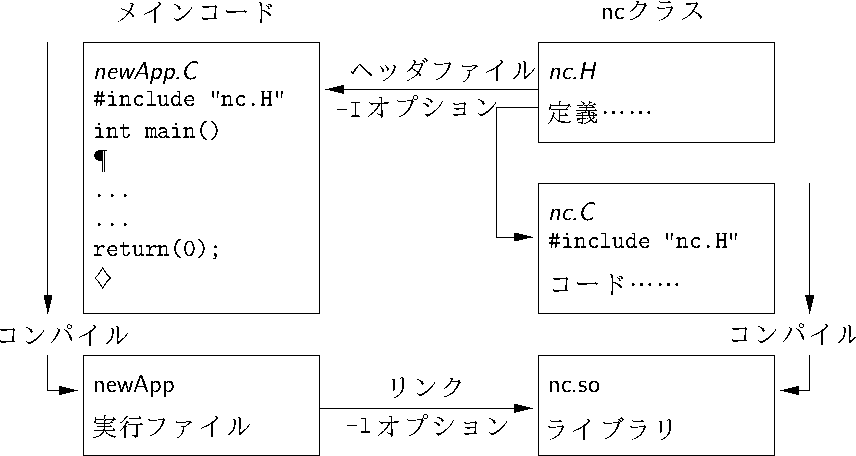
\includegraphics{fig-3-1}
 \caption{ヘッダファイル,ソースファイル,コンパイル,リンク}
 \label{fig:3.1}
\end{figure}


\subsection{ヘッダ\OFpath{.H}ファイル}
\label{ssec:3.2.1}
エラーチェックをおこなうにあたって,
コンパイルするコードの部分がどのクラスで用いられるか,
また実際の操作でどのように振舞うかを認識しなければなりません.
それゆえ,(例えば\OFpath{nc.H}のような) \OFpath{.H}ファイル拡張子をもつ
ヘッダファイルによってクラス宣言が必要です.
このようなヘッダファイルにはクラス名とその機能が記述されています.

このファイルは,クラスを用いるあらゆるコード
(クラス宣言のためのコードも含め)の最初の部分に置きます.
\OFpath{.C}コードではどの部分でいくつのクラスを用いてもかまいませんが,
かならずクラス宣言のために\OFpath{.H}ファイルではじめる必要があります.
クラスは他のクラスのリソースとして使うことができますが,
その場合も関連付けた\OFpath{.H}ファイルではじめます.
クラスヒエラルキを再帰的に検索することで,
結局,上位\OFpath{.C}コードが
\index{いぞん@依存}%
依存しているクラス
(これらの\OFpath{.H}ファイルはdependencyとよばれる) で,
すべてのクラスに関するヘッダファイルのリストを
コンパイルすることができます.
\index{いぞんリスト@依存リスト}%
依存リストがあればコンパイラはソースファイルが
最終コンパイル以来アップデートされているかどうかチェックでき,
選択的に必要な部分だけコンパイルできます.

ヘッダファイルは,例えば
\begin{OFverbatim}[file]
# include "otherHeader.H";
\end{OFverbatim}
のような\ 
\index{# include@\verb+# include+!C++こうぶん@C++構文}%
\index{C++こうぶん@C++構文!# include@\verb+# include+}%
\verb|# include|命令文を使ったコードに含まれていますが,
このようなコードはコンパイラに特定のファイルを読ませるために
現在のファイルの読み込みを一時中断させます.
すべての内蔵コードはヘッダファイルに入れること,
コード可読性を高めるためにメインコードにrelevant locationに
含めることができます.
例えば多くのOpenFOAMアプリケーションでは,
作成フィールドや読み込みフィールドの入力データのコードはコードの始めに
\OFpath{createFields.H}と名づけられたファイルに含まれます.
この方法では,ヘッダファイルは単独でクラスの宣言として
使われるだけではありません.
以下のようなその他の機能とともに依存リストファイルを
維持管理するタスクを実行するのが\OFtool{wmake}なのです.
\begin{itemize}
 \item ソースファイルと,それらが依存しているファイルの
       依存関係リストの自動作成と管理
 \item マルチ・プラットフォームコンパイル適切なディレクトリ構造を通じて
       ハンドルされたマルチプラットフォームでのコンパイルとリンク
 \item マルチ・ランゲージコンパイルとCやC++やJava等のリンケージ
 \item CやC++,Javaのようなマルチ言語でのコンパイルとリンク
 \item デバッグや最適化,並列処理,分析といった
       マルチオプションでのコンパイルとリンク
 \item lex,yacc,IDL,MOCといった,ソースコードの作成プログラムのサポート
 \item ソースファイルリストの簡潔なシンタックス
 \item 新規のコードリストのソースファイルリストの自動生成
 \item 多重分割あるいは静的ライブラリの簡潔なハンドリング
 \item 新しいタイプのマシンへの拡張性
 \item \texttt{make};\texttt{sh},\texttt{ksh}または\texttt{csh};
       \texttt{lex},\texttt{cc}をもついかなるマシンでの
       作業に対する優れた移植性
 \item Apollo,SUN,SGI,HP (HPUX),Compaq (DEC),IBM (AIX),Cray,Ardent,
       Stardent,PC Linux,PPC Linux,NEC,SX4,Fujitsu VP1000での動作確認
\end{itemize}


\subsection{\OFtool{wmake}によるコンパイル}
\label{ssec:3.2.2}
OpenFOAMのアプリケーションは各アプリケーションのソースコードが
そのアプリケーション名のディレクトリに置かれるという
一般的決まりで編成されます.
最上位ソースファイルはアプリケーション名に拡張子\OFpath{.C}をつけます.
例えば,newAppというアプリケーションのソースコードは
\autoref{fig:3.2}に示すようにnewAppのディレクトリに存在し,
最上位ファイルは\OFpath{newApp.C}となります.


\begin{figure}[ht]
 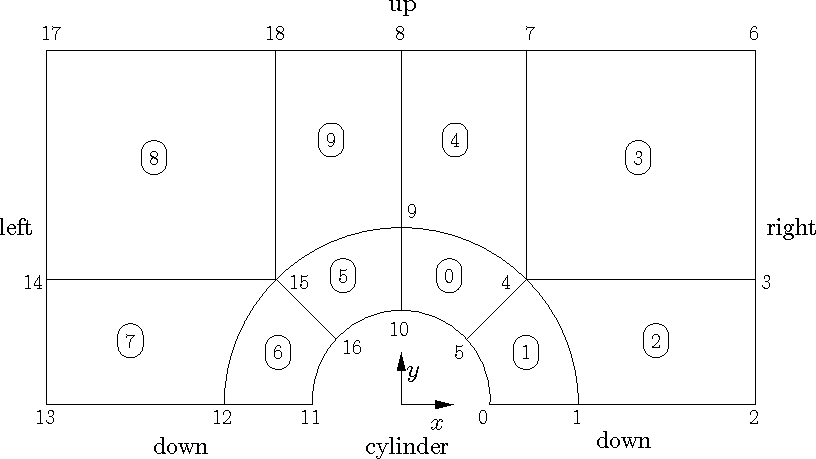
\includegraphics{fig-3-2}
 \caption{アプリケーションのディレクトリ構成}
 \label{fig:3.2}
\end{figure}


ディレクトリは
\index{options@\OFpath{options}!ファイル}%
\index{ファイル!options@\OFpath{options}}%
\OFpath{options}と
\index{files@\OFpath{files}!ファイル}%
\index{ファイル!files@\OFpath{files}}%
\OFpath{files}の二つのファイルを含んだ
\index{Make@\OFpath{Make}!ディレクトリ}%
\index{ディレクトリ!Make@\OFpath{Make}}%
\OFpath{Make}というサブディレクトリももっており,それについては次節で述べます.

\subsubsection{ヘッダの読み込み}
\label{sssec:3.2.2.1}
コンパイラは,以下の順で
\OFtool{wmake}で\verb|−I|オプションが指定されたヘッダファイルを検索します.
\begin{enumerate}
 \item \OFpath{\$WM\_PROJECT\_DIR/src/OpenFOAM/lnInclude}ディレクトリ
 \item \OFpath{newApp/lnInclude}のようなローカルディレクトリ
 \item \OFpath{newApp}のようなローカルディレクトリ
 \item \OFpath{/usr/X11/include}や\OFpath{\$(MPICH\_ARCH\_PATH)/include}のように,
\index{wmake@\OFtool{wmake}!プラットフォーム}%
       プラットフォームに依存する
       \OFpath{\$WM\_PROJECT\_DIR/wmake/rules/\$WM\_ARCH/}ディレクトリの中の
       ファイルに設定されているパス
 \item \verb|-I|オプションをもつ\OFpath{Make/options}ファイルの中で
       明確に指定されている他のディレクトリ
\end{enumerate}
\OFpath{Make/options}ファイルは構文を使っているヘッダファイルを
配置するためのフルディレクトリパスを含みます.
\begin{OFverbatim}[file]
EXE_INC = \
    -I<directoryPath1> \
    -I<directoryPath2> \
    ...                \
    -I<directoryPathN>
\end{OFverbatim}
ディレクトリ名は頭に\verb|-I|をつけ,
各行では\verb|EXE_INC|を続けるために構文は\verb|\|を使い,
最終記入後は\verb|\|をつけないことに注意してください.

\subsubsection{ライブラリへのリンク}
\label{sssec:3.2.2.2}
コンパイラは,以下の\OFtool{wmake}の\verb|-L|オプションで指定された
ディレクトリパスのオブジェクトライブラリファイルにリンクします.
\begin{enumerate}
 \item \OFpath{\$FOAM\_LIBBIN}ディレクトリ
 \item \OFpath{\$WM\_DIR/rules/\$WM\_ARCH/}デイレクトリの中に設定された
       機種に依存するパス,例えば,\OFpath{/usr/X11/}や\OFpath{\$(MPICH\_ARCH\_PATH)/lib}
 \item \OFpath{Make/options}ファイルで指定された他のディレクトリ
\end{enumerate}
リンクされる実際のライブラリファイルは\verb|-l|オプションで指定し,
接頭辞\OFpath{lib},ライブラリファイルの拡張子\OFpath{.so}を
外さなければなりません.
例えばライブラリ\OFpath{libnew.so}はフラグ\verb|-lnew|に含まれます.

デフォルトでは,\OFtool{wmake}は以下のライブラリをロードするようになっています
\begin{enumerate}
 \item \OFpath{\$FOAM\_LIBBIN}ディレクトリからの\OFpath{libOpenFOAM.so}ライブラリ
 \item \OFpath{\$WM\_DIR/rules/\$WM\_ARCH/}ディレクトリの中のファイルに設定された
       機種に依存するライブラリ,
       例えば,\OFpath{/usr/X11/lib}における\OFpath{libm.so}や,
       \OFpath{\$(LAM ARCH PATH)/lib}における\OFpath{liblam.so}
 \item \OFpath{Make/options}ファイルで指定された他のライブラリ
\end{enumerate}
\OFpath{Make/options}ファイルは構文を使っているヘッダファイルを
おくための全ディレクトリパスを含みます.
\begin{OFverbatim}[file]
EXE_LIBS = \
    -L<libraryPath1> \
    -L<libraryPath2> \
    ...              \
    -L<libraryPathN> \
    -l<library1>     \
    -l<library2>     \
    ...              \
    -l<libraryN>
\end{OFverbatim}
繰り返しになりますが,ディレクトリパスは頭に\verb|-L|フラグを付け,
ライブラリ名は頭に\verb|-l|フラグをつけます.

\subsubsection{コンパイルすべきソースファイル}
\label{sssec:3.2.2.3}
コンパイラはコンパイルすべき\OFpath{.C}ソースファイルのリストが必要です.
リストはメインの\OFpath{.C}ファイルだけではなく
特定のアプリケーションのために生成されるがクラスライブラリの中に
含まれない他のソースファイルも含まれなければなりません.
例えば,新しいクラスを作成したり,
特定のアプリケーション用のクラスに
新しい機能をつけくわえることができます.
\OFpath{.C}ソースファイルのフルリストは
\index{Make/files@\OFpath{Make/files}!ファイル}%
\index{ファイル!Make/files@\OFpath{Make/files}}%
\OFpath{Make/files}ファイルに
含む必要があります.当然,アプリケーションは多くなるので,
フルリストには (例えば前述のアプリケーション例における
\OFpath{newApp.C}のような) メイン\OFpath{.C}ファイルの名前だけを入れます.
\OFpath{Make/files}ファイルは\verb|EXE =|構文によって
指定されたコンパイル済み実行ファイルの名前とフルパスも含みます.
一般的な決まりではnewAppのようにアプリケーション名をつけることが
規定されています.
OpenFOAMのリリースにはパスのために便利な二つの選択肢があります.
標準的なリリースではアプリケーションは\OFpath{\$FOAM\_APPBIN}に
保存されますが,ユーザにより開発されたアプリケーションは
\OFpath{\$FOAM\_USER\_APPBIN}に保存されます.

もしアプリケーションを開発したら,
個人のOpenFOAMアプリケーションのためのソースコードを含む
\OFpath{\$WM\_PROJECT\_USER\_DIR}ディレクトリに
アプリケーションサブディレクトリを作ることをお薦めします.
スタンダードアプリケーションと同様に
各OpenFOAMアプリケーションのソースコードも
各ディレクトリ内に保存しておいてください.
ユーザーアプリケーションとスタンダードリリースのものの違いは
\OFpath{Make/files}ファイルが\OFpath{\$FOAM\_USER\_APPBIN}ディレクトリ内に
書き込まれている実行可能ファイルを指定していることだけです.
例としての\OFpath{Make/files}を以下に記載します.
\begin{OFverbatim}[file]
newApp.C

EXE = $(FOAM_USER_APPBIN)/newApp
\end{OFverbatim}%$

\subsubsection{\OFtool{wmake}の実行}
\label{sssec:3.2.2.4}
\OFtool{wmake}のスクリプトは以下のように入力することで実行されます.
\begin{OFverbatim}[terminal]
wmake <optionalArguments> <optionalDirectory>
\end{OFverbatim}
\verb|<optionalDirectory>| はコンパイルしようとしているアプリケーションの
ディレクトリパスです.
通常,\verb|<optionalDirectory>| が省略可能な場合には
\OFtool{wmake}はコンパイル中のアプリケーションのディレクトリ内から実行されます.


アプリケーションファイルを作成したい場合には
\verb|<optionalArguments>|は必要ありません.
しかし\verb|<optionalArguments>|は\autoref{tbl:3.1}に示すように
ライブラリ等の作成の際には指定されることになります.


\begin{table}[ht]
 %#! platex UserGuideJa
\begin{tabular}{ll}
 Argument & コンパイルの種類 \\
 \hline
 \tblstrut
 \texttt{lib} & 静的にリンクされたライブラリの作成 \\
 \texttt{libso} & 動的にリンクされたライブラリの作成 \\
 \texttt{libo} & 静的にリンクされたオブジェクトファイルライブラリの作成 \\
 \texttt{jar} & JAVAアーカイブの作成 \\
 \texttt{exe} & 特定のプロジェクトから独立したアプリケーションの作成 \\
 \hline
\end{tabular}

 \caption{\OFtool{wmake}のコンパイルオプション}
 \label{tbl:3.1}
\end{table}


\subsubsection{\OFtool{wmake}の環境変数}
\label{sssec:3.2.2.5}
参考として,\OFtool{wmake}で使われる環境変数の設定を
\autoref{tbl:3.2}に示します.


\begin{table}[ht]
 %#! platex UserGuideJa
\begin{tabularx}{\textwidth}{lX}
 主なパス & \\
 \hline
\index{WM PROJECT INST DIR@\string\OFenv{WM\_PROJECT\_INST\_DIR}!かんきょうへんすう@環境変数}%
\index{かんきょうへんすう@環境変数!WM PROJECT INST DIR@\string\OFenv{WM\_PROJECT\_INST\_DIR}}%
 \OFenv{\$WM\_PROJECT\_INST\_DIR}
 & インストールディレクトリへのフルパス,例:\OFpath{\$HOME/OpenFOAM} \\
\index{WM PROJECT@\string\OFenv{WM\_PROJECT}!かんきょうへんすう@環境変数}%
\index{かんきょうへんすう@環境変数!WM PROJECT@\string\OFenv{WM\_PROJECT}}%
 \OFenv{\$WM\_PROJECT}
 & コンパイルされたプロジェクトの名前:\texttt{OpenFOAM} \\
\index{WM PROJECT VERSION@\string\OFenv{WM\_PROJECT\_VERSION}!かんきょうへんすう@環境変数}%
\index{かんきょうへんすう@環境変数!WM PROJECT VERSION@\string\OFenv{WM\_PROJECT\_VERSION}}%
 \OFenv{\$WM\_PROJECT\_VERSION}
 & コンパイルされたプロジェクトのバージョン:\texttt{\OFversion} \\
\index{WM PROJECT DIR@\string\OFenv{WM\_PROJECT\_DIR}!かんきょうへんすう@環境変数}%
\index{かんきょうへんすう@環境変数!WM PROJECT DIR@\string\OFenv{WM\_PROJECT\_DIR}}%
 \OFenv{\$WM\_PROJECT\_DIR}
 & OpenFOAMのバイナリ実行ファイル置き場へのフルパス,\hfil\break
     例:\OFpath{\$HOME/OpenFOAM/OpenFOAM-\OFversion} \\
\index{WM PROJECT USER DIR@\string\OFenv{WM\_PROJECT\_USER\_DIR}!かんきょうへんすう@環境変数}%
\index{かんきょうへんすう@環境変数!WM PROJECT USER DIR@\string\OFenv{WM\_PROJECT\_USER\_DIR}}%
 \OFenv{\$WM\_PROJECT\_USER\_DIR}
 & ユーザのバイナリ実行ファイル置き場へのフルパス,\hfil\break
     例:\OFpath{\$HOME/OpenFOAM/\${USER}-\OFversion} \\
 \\
 その他のパスと設定 & \\
 \hline
\index{WM ARCH@\string\OFenv{WM\_ARCH}!かんきょうへんすう@環境変数}%
\index{かんきょうへんすう@環境変数!WM ARCH@\string\OFenv{WM\_ARCH}}%
 \OFenv{\$WM\_ARCH}
 & マシン・アーキテクチャ:
     \texttt{Linux}, \texttt{SunOS} \\
\index{WM ARCH OPTION@\string\OFenv{WM\_ARCH\_OPTION}!かんきょうへんすう@環境変数}%
\index{かんきょうへんすう@環境変数!WM ARCH OPTION@\string\OFenv{WM\_ARCH\_OPTION}}%
 \OFenv{\$WM\_ARCH\_OPTION}
 & \texttt{32}あるいは\texttt{64}ビットのアーキテクチャ \\
\index{WM COMPILER@\string\OFenv{WM\_COMPILER}!かんきょうへんすう@環境変数}%
\index{かんきょうへんすう@環境変数!WM COMPILER@\string\OFenv{WM\_COMPILER}}%
 \OFenv{\$WM\_COMPILER}
 & 使用するコンパイラ:\texttt{Gcc45} - \textsf{gcc} 4.5+, \texttt{ICC} - Intel \\
\index{WM COMPILER DIR@\string\OFenv{WM\_COMPILER\_DIR}!かんきょうへんすう@環境変数}%
\index{かんきょうへんすう@環境変数!WM COMPILER DIR@\string\OFenv{WM\_COMPILER\_DIR}}%
 \OFenv{\$WM\_COMPILER\_DIR}
 & コンパイラインストールディレクトリ \\
\index{WM COMPILER BIN@\string\OFenv{WM\_COMPILER\_BIN}!かんきょうへんすう@環境変数}%
\index{かんきょうへんすう@環境変数!WM COMPILER BIN@\string\OFenv{WM\_COMPILER\_BIN}}%
 \OFenv{\$WM\_COMPILER\_BIN}
 & コンパイラインストールバイナリ:\OFpath{\$WM\_COMPILER\_BIN/bin} \\
\index{WM COMPILER LIB@\string\OFenv{WM\_COMPILER\_LIB}!かんきょうへんすう@環境変数}%
\index{かんきょうへんすう@環境変数!WM COMPILER LIB@\string\OFenv{WM\_COMPILER\_LIB}}%
 \OFenv{\$WM\_COMPILER\_LIB}
 & コンパイラインストールライブラリ:\OFpath{\$WM\_COMPILER\_BIN/lib} \\
\index{WM COMPILE OPTION@\string\OFenv{WM\_COMPILE\_OPTION}!かんきょうへんすう@環境変数}%
\index{かんきょうへんすう@環境変数!WM COMPILE OPTION@\string\OFenv{WM\_COMPILE\_OPTION}}%
 \OFenv{\$WM\_COMPILE\_OPTION}
 & コンパイルオプション:\texttt{Debug} - debugging, \texttt{Opt} optimisation. \\
\index{WM DIR@\string\OFenv{WM\_DIR}!かんきょうへんすう@環境変数}%
\index{かんきょうへんすう@環境変数!WM DIR@\string\OFenv{WM\_DIR}}%
 \OFenv{\$WM\_DIR}
 & wmakeディレクトリのフルパス \\
\index{WM MPLIB@\string\OFenv{WM\_MPLIB}!かんきょうへんすう@環境変数}%
\index{かんきょうへんすう@環境変数!WM MPLIB@\string\OFenv{WM\_MPLIB}}%
 \OFenv{\$WM\_MPLIB}
 & 並列通信ライブラリ:\texttt{LAM},\texttt{MPI},\texttt{MPICH},\texttt{PVM} \\
\index{WM OPTIONS@\string\OFenv{WM\_OPTIONS}!かんきょうへんすう@環境変数}%
\index{かんきょうへんすう@環境変数!WM OPTIONS@\string\OFenv{WM\_OPTIONS}}%
 \OFenv{\$WM\_OPTIONS}
 & $=$ \OFenv{\$WM\_ARCH\$WM\_COMPILER...}\hfill\break
     \null\hfill\OFenv{...\$WM\_COMPILE\_OPTION\$WM\_MPLIB},\break
     例:\texttt{linuxGcc3OptMPICH} \\
\index{WM PRECISION OPTION@\string\OFenv{WM\_PRECISION\_OPTION}!かんきょうへんすう@環境変数}%
\index{かんきょうへんすう@環境変数!WM PRECISION OPTION@\string\OFenv{WM\_PRECISIO\_OPTION}}%
 \OFenv{\$WM\_PRECISION\_OPTION}
 & コンパイルされたバイナリの精度,\texttt{SP}なら単精度,もしくは,\texttt{DP}なら倍精度 \\
 \hline
\end{tabularx}

 \caption{\OFtool{wmake}の環境変数の設定}
 \label{tbl:3.2}
\end{table}


\subsection{依存リストの削除:\OFtool{wclean}と\OFtool{rmdepall}}
\label{ssec:3.2.3}
実行に際して,例題における\OFpath{newApp.dep}のように,
\OFtool{wmake}は拡張子として\OFpath{.dep}をもった依存関係のリストファイルを構築し,
\OFpath{Make/\$WM\_OPTIONS}ディレクトリの中にファイルのリストを格納します.
コードを変更してmakeした後などこれらファイルを除去したい場合には,
\index{wclean@\OFtool{wclean}!スクリプト/エイリアス}%
\index{スクリプト/エイリアス!wclean@\OFtool{wclean}}%
\OFtool{wclean}を入力してスクリプトを実行します.
\begin{OFverbatim}[terminal]
wclean <optionalArguments> <optionalDirectory>
\end{OFverbatim}
さらに,\verb|<optionalDirectory>|はコンパイルされるアプリケーションの
ディレクトリへのパスです.
通常,パスが省略できる場合にはwcleanはアプリケーションの
ディレクトリ範囲内で実行されます.
もし\OFpath{Make}ディレクトリから依存ファイルとファイルを削除したい場合には,
\verb|<optionalArguments>|は必要ありません.
しかしもしlibが\verb|<optionalArguments>|に指定されていたら
ローカルの\OFpath{InInclude}ディレクトリも削除される必要があります.

追加のスクリプト,
\index{rmdepall@\OFtool{rmdepall}!スクリプト/エイリアス}%
\index{スクリプト/エイリアス!rmdepall@\OFtool{rmdepall}}%
\OFtool{rmdepall}は実行時に,
再帰的にディレクトリツリー下の依存関係にあるすべての
\OFpath{.dep}ファイルを除去します.
これはOpenFOAMのライブラリが更新されたときには有効な方法です.


\subsection{コンパイルの例:pisoFoamアプリケーション}
\label{ssec:3.2.4}
アプリケーション\OFtool{pisoFoam}のソースコードは
\OFpath{\$FOAM\_APP/solvers/incompressible/pisoFoam}ディレクトリ内にあり,
最上位ソースファイルは\OFpath{pisoFoam.C}という名前です.
\OFpath{pisoFoam.C}ソースコードは
\begin{OFverbatim}[file, linenum]
/*---------------------------------------------------------------------------*\
  =========                 |
  \\      /  F ield         | OpenFOAM: The Open Source CFD Toolbox
   \\    /   O peration     |
    \\  /    A nd           | Copyright (C) 1991-2010 OpenCFD Ltd.
     \\/     M anipulation  |
-------------------------------------------------------------------------------
License
    This file is part of OpenFOAM.

    OpenFOAM is free software: you can redistribute it and/or modify it
    under the terms of the GNU General Public License as published by
    the Free Software Foundation, either version 3 of the License, or
    (at your option) any later version.

    OpenFOAM is distributed in the hope that it will be useful, but WITHOUT
    ANY WARRANTY; without even the implied warranty of MERCHANTABILITY or
    FITNESS FOR A PARTICULAR PURPOSE.  See the GNU General Public License
    for more details.

    You should have received a copy of the GNU General Public License
    along with OpenFOAM.  If not, see <http://www.gnu.org/licenses/>.

Application
    pisoFoam

Description
    Transient solver for incompressible flow.

    Turbulence modelling is generic, i.e. laminar, RAS or LES may be selected.

\*---------------------------------------------------------------------------*/

#include "fvCFD.H"
#include "singlePhaseTransportModel.H"
#include "turbulenceModel.H"

// * * * * * * * * * * * * * * * * * * * * * * * * * * * * * * * * * * * * * //

int main(int argc, char *argv[])
{
    #include "setRootCase.H"

    #include "createTime.H"
    #include "createMesh.H"
    #include "createFields.H"
    #include "initContinuityErrs.H"

    // * * * * * * * * * * * * * * * * * * * * * * * * * * * * * * * * * * * //

    Info<< "\nStarting time loop\n" << endl;

    while (runTime.loop())
    {
        Info<< "Time = " << runTime.timeName() << nl << endl;

        #include "readPISOControls.H"
        #include "CourantNo.H"

        // Pressure-velocity PISO corrector
        {
            // Momentum predictor

            fvVectorMatrix UEqn
            (
                fvm::ddt(U)
              + fvm::div(phi, U)
              + turbulence->divDevReff(U)
            );

            UEqn.relax();

            if (momentumPredictor)
            {
                solve(UEqn == -fvc::grad(p));
            }

            // --- PISO loop

            for (int corr=0; corr<nCorr; corr++)
            {
                volScalarField rUA = 1.0/UEqn.A();

                U = rUA*UEqn.H();
                phi = (fvc::interpolate(U) & mesh.Sf())
                    + fvc::ddtPhiCorr(rUA, U, phi);

                adjustPhi(phi, U, p);

                // Non-orthogonal pressure corrector loop
                for (int nonOrth=0; nonOrth<=nNonOrthCorr; nonOrth++)
                {
                    // Pressure corrector

                    fvScalarMatrix pEqn
                    (
                        fvm::laplacian(rUA, p) == fvc::div(phi)
                    );

                    pEqn.setReference(pRefCell, pRefValue);

                    if
                    (
                        corr == nCorr-1
                     && nonOrth == nNonOrthCorr
                    )
                    {
                        pEqn.solve(mesh.solver("pFinal"));
                    }
                    else
                    {
                        pEqn.solve();
                    }

                    if (nonOrth == nNonOrthCorr)
                    {
                        phi -= pEqn.flux();
                    }
                }

                #include "continuityErrs.H"

                U -= rUA*fvc::grad(p);
                U.correctBoundaryConditions();
            }
        }

        turbulence->correct();

        runTime.write();

        Info<< "ExecutionTime = " << runTime.elapsedCpuTime() << " s"
            << "  ClockTime = " << runTime.elapsedClockTime() << " s"
            << nl << endl;
    }

    Info<< "End\n" << endl;

    return 0;
}


// ************************************************************************* //
\end{OFverbatim}
コードはアプリケーションを説明している記述で始まり,
この中で1行の
\index{コメント}%
コメントは\ 
\index{//@\verb+//+!C++こうぶん@C++構文}%
\index{C++こうぶん@C++構文!//@\verb+//+}%
\verb|//| で,
複数行にわたる
\index{コメント}%
コメントは\ 
\index{/*...*/@\verb+/*...*/+!C++こうぶん@C++構文}%
\index{C++こうぶん@C++構文!/*...*/@\verb+/*...*/+}%
\verb|/*...*/| で記述されます.それに続き,
コードはコンパイラに現在のファイルの読み込みを一時停止させ,
\OFpath{pisoFoam.C}に\OFpath{fvCFD.H}を読み込ませるための
例えば\verb|#include "fvCFD.H"|のような
様々な\ 
\index{# include@\verb+# include+!C++こうぶん@C++構文}%
\index{C++こうぶん@C++構文!# include@\verb+# include+}%
\verb|# include|命令文を含んでいます.

\OFtool{pisoFoam}は\OFclass{incompressibleRASModels}や
\OFclass{incompressibleLESModels}や
\OFclass{incompressibleTransportModels}ライブラリを提供し,
それゆえ\verb|EXE_INC = -I...|オプションとライブラリにリンクする
\verb|EXE_LIBS = -l...|オプションにより
指定されるヘッダファイルが必要となります.
\OFpath{Make/options}はそれゆえ以下のようになります.
\begin{OFverbatim}[file, linenum]
EXE_INC = \
    -I$(LIB_SRC)/turbulenceModels/incompressible/turbulenceModel \
    -I$(LIB_SRC)/transportModels \
    -I$(LIB_SRC)/transportModels/incompressible/singlePhaseTransportModel \
    -I$(LIB_SRC)/finiteVolume/lnInclude

EXE_LIBS = \
    -lincompressibleRASModels \
    -lincompressibleLESModels \
    -lincompressibleTransportModels \
    -lfiniteVolume \
    -lmeshTools
\end{OFverbatim}
\OFtool{pisoFoam}は\OFpath{pisoFoam.C}ソースしか含まず,
実行ファイルはすべての標準的なアプリケーションと同様に
\OFpath{\$FOAM\_APPBIN}に書き込まれます.
\OFpath{Make/files}はそれゆえ以下のようになります.
\begin{OFverbatim}[file, linenum]
pisoFoam.C

EXE = $(FOAM_APPBIN)/pisoFoam
\end{OFverbatim}%$
\OFpath{\$FOAM\_CFD/pisoFoam}ディレクトリで\verb|wmake|とタイプすれば
\OFtool{pisoFoam}をコンパイルできます.

コードはコンパイルされ以下のようなメッセージをが作成されます.
\begin{OFverbatim}[file]
Making dependency list for source file pisoFoam.C
SOURCE DIR=.
SOURCE=pisoFoam.C ;
g++ -DFOAM EXCEPTION -Dlinux -DlinuxOptMPICH
-DscalarMachine -DoptSolvers -DPARALLEL -DUSEMPI -Wall -O2 -DNoRepository
-ftemplate-depth-17 -I.../OpenFOAM/OpenFOAM-1.7.1/src/OpenFOAM/lnInclude
-IlnInclude
-I.
......
-lmpich -L/usr/X11/lib -lm
-o .../OpenFOAM/OpenFOAM-1.7.1/applications/bin/linuxOptMPICH/pisoFoam
\end{OFverbatim}
再コンパイルすることも可能ですが,
実行ファイルが最新でコンパイルする必要がないというときには
以下のようなメッセージが返ってきます.
\begin{OFverbatim}[file]
make: Nothing to be done for `allFiles'.
make: `Make/linuxOptMPICH/dependencies' is up to date.
make: `.../OpenFOAM/OpenFOAM-1.7.1/applications/bin/linuxOptMPICH/pisoFoam'
is up to date.
\end{OFverbatim}

\begin{OFverbatim}[terminal]
wclean
\end{OFverbatim}
を使って依存リストを削除し,
\OFtool{wmake}を起動することでゼロからアプリケーションをコンパイルできます.


\subsection{デバッグメッセージと最適化スイッチ}
\label{ssec:3.2.5}
OpenFOAMは,実行時にメッセージを出力するシステムを提供しており,
これらのメッセージの多くは,OpenFOAMのケースの実行時に遭遇する問題のデバッグに役立ちます.
そのスイッチは\OFpath{\$WM\_PROJECT\_DIR/etc/controlDict}ファイルの
中にあり,設定を変更したい場合には,
\OFpath{\$HOME}ディレクトリに (例えば
\OFpath{\$HOME/.OpenFOAM/1.7.1/controlDict}ファイルのように) コピーを
作成します.スイッチが可能なリストは非常に多く,
\OFtool{foamDebugSwitches}アプリケーションを実行することにより閲覧できます.
スイッチのほとんどは,クラスまたは機能性のレンジと一致しており,
設定を1にすることにより,
\OFdictionary{controlDict}ファイルの中にあるそれ自身により変更できます.
例えば,OpenFOAMでは,\OFkeyword{dimensionSet}スイッチを1に設定することにより,
すべての計算におけるディメンションをチェックする機能があります.
\autoref{tbl:3.3}に示すものは
より高機能にメッセージをコントロールできるスイッチです.

加えて,いくつかのオペレーションと最適化をコントロールする
スイッチがあります.これらのスイッチについても
\autoref{tbl:3.3}に示します.
特に重要なものは\OFkeyword{fileModificationSkew}であり,
OpenFOAMでは,変更をチェックするために
データファイルの書き込み時間をスキャンしています.
異なるマシンでクロックの設定に不整合が生じた状態で
NFSを実行すると,先駆けしてフィールドデータの修正が表示されます.
このことは,OpenFOAMが新規に修正されたとしてファイルを閲覧する場合と,
このデータを再読み込みしようとする場合には
問題を引き起こすことになります.
キーワード\OFkeyword{fileModificationSkew}は秒単位の時間であり,
OpenFOAMは,ファイルが新しく修正されたかどうか調べるときには,
ファイルの書き込み時間から差し引きます.


\begin{table}[ht]
 %#! platex UserGuideJa
\begin{tabularx}{\textwidth}{lX}
 \multicolumn{2}{l}{ハイレベルデバッグスイッチ - サブディクショナリ \OFdictionary{DebugSwitches}} \\
 \hline
 \texttt{level} & OpenFOAMのデバッグメッセージの全体のレベル - - 0, 1, 2の3レベル \\
 \texttt{lduMatrix} & 実行中のソルバの収束メッセージ - 0, 1, 2の3レベル \\
 \\
 \multicolumn{2}{l}{最適化スイッチ - サブディクショナリ \OFdictionary{OptimisationSwitches}} \\
 \hline
 \index{fileModificationSkew@\texttt{fileModificationSkew}!キーワード}%
 \index{キーワード!fileModificationSkew@\texttt{fileModificationSkew}}%
 \texttt{fileModificationSkew} & NFSの上でNFSのアップデートの最大遅れと
     OpenFOAM実行のための差分クロックより長く設定すべき時間(秒). \\
 \index{fileModificationChecking@\texttt{fileModificationChecking}!キーワード}%
 \index{キーワード!fileModificationChecking@\texttt{fileModificationChecking}}%
 \texttt{fileModificationChecking} & シミュレーション中にファイルが変更されたか
     どうかをチェックする方法であり,
	 \index{timeStamp@\OFkeyword{timeStamp}!キーワードエントリ}%
	 \index{キーワードエントリ!timeStamp@\OFkeyword{timeStamp}}%
	 \OFkeyword{timeStamp}を読む,
     または
	 \index{inotify@\OFkeyword{inotify}!キーワードエントリ}%
	 \index{キーワードエントリ!inotify@\OFkeyword{inotify}}%
	 \OFkeyword{inotify}(通知しない),
     あるいはマスタ・ノードに存在するデータのみを読み込む
	 \index{timeStampMaster@\OFkeyword{timeStampMaster}!キーワードエントリ}%
	 \index{キーワードエントリ!timeStampMaster@\OFkeyword{timeStampMaster}}%
	 \OFkeyword{timeStampMaster},
     \index{inotifyMaster@\OFkeyword{inotifyMaster}!キーワードエントリ}%
     \index{キーワードエントリ!inotifyMaster@\OFkeyword{inotifyMaster}}%
	 \OFkeyword{inotifyMaster}があります. \\
\index{commsType@\texttt{commsType}!キーワード}%
\index{キーワード!commsType@\texttt{commsType}}%
\texttt{commsType} & 並列計算の通信方法.\OFkeyword{nonBlocking},
     \OFkeyword{scheduled},\OFkeyword{blocking}. \\
	 \index{nonBlocking@\OFkeyword{nonBlocking}!キーワードエントリ}%
	 \index{キーワードエントリ!nonBlocking@\OFkeyword{nonBlocking}}%
	 \index{scheduled@\OFkeyword{scheduled}!キーワードエントリ}%
	 \index{キーワードエントリ!scheduled@\OFkeyword{scheduled}}%
	 \index{blocking@\OFkeyword{blocking}!キーワードエントリ}%
	 \index{キーワードエントリ!blocking@\OFkeyword{blocking}}%
\index{floatTransfer@\texttt{floatTransfer}!キーワード}%
\index{キーワード!floatTransfer@\texttt{floatTransfer}}%
\texttt{floatTransfer} & \OFkeyword{1}とすると,
     転送の前に数値を\OFkeyword{float}の精度に丸めます.デフォルトは\OFkeyword{0}です. \\
 \texttt{nProcsSimpleSum} & 並列処理のために全領域の和を最適化します.
     階層和は線形和(デフォルトで16)よりよく機能し,
     プロセッサの数を設定します. \\
 \hline
\end{tabularx}

 \caption{ランタイムメッセージスイッチ}
 \label{tbl:3.3}
\end{table}


\subsection{現在のアプリケーションへの新しいユーザ定義ライブラリのリンク}
\label{ssec:3.2.6}
タイトルのような状況は,
新しいライブラリ (例えば\OFemph{new}) を作成するとき,
新しい宣言およびアプリケーションのレンジを越えて
ライブラリの中に入れ込みたい場合に生じることが考えられます.
例えば,ユーザーが新規の境界条件を作成し,\OFemph{new}の中でコンパイルし,
ソルバのアプリケーションや,
前および後処理用のユーティリティ,
メッシュツール等々の範囲で認識させる必要があることがあります.
通常の環境下では,ユーザはすべてのアプリケーションを,
リンクさせるために\OFemph{new}で再コンパイルする必要があります.

その代わりにOpenFOAMでは,
一つもしくは複数の共有オブジェクトライブラリを
実行時に動的にリンクさせるメカニズムを採用しています.
そのためには,ただ単に\OFpath{controlDict}に
オプションのキーワードである
\index{libs@\OFkeyword{libs}!キーワード}%
\index{キーワード!libs@\OFkeyword{libs}}%
\OFkeyword{libs}を追加し,
ライブラリの完全なファイル名を引用符付き文字列のエントリとして
リストに入力すればすればよいだけです.
たとえば\OFemph{new1}と\OFemph{new2}というライブラリを実行時にリンクしたいなら,
\OFpath{controlDict}に以下を書き加えます.
\begin{OFverbatim}[file]
libs
(
    "libnew1.so"
    "libnew2.so"
);
\end{OFverbatim}



\section{アプリケーションの実行}
\label{sec:3.3}
各アプリケーションは,
ターミナルのコマンドラインから実行されるようになっており,
個別のケースに関連したデータファイルのセットの書き込みと
読み込みが行われるようになっています.
ケースに関するデータファイルは
\autoref{sec:4.1}で述べているように,
ケースの後に名前をつけられたディレクトリの中に格納されており,
ここではフルパスをもつディレクトリ名は
一般名\OFpath{<caseDir>}としています.

どのアプリケーションにおいても,
コマンドラインの入力フォームはコマンドラインで
アプリーション名に\verb|-help|オプションをつけて
入力するだけで見つけられます.例えば
\begin{OFverbatim}[terminal]
blockMesh -help
\end{OFverbatim}
と入力すると以下を含むデータが返ってきます.
\begin{OFverbatim}[terminal]
Usage: blockMesh [-region region name] [-case dir] [-blockTopology]
    [-help] [-doc] [-srcDoc]
\end{OFverbatim}
角括弧\texttt{[ ]}内の引数はオプショナルフラグです.
アプリケーションがケースディレクトリ内で実行されると,
そのケースを作動します.
あるいは,\texttt{-case}~\OFpath{<caseDir>}オプションでは,
直接ファイリングシステムで
どこからでもアプリケーションを実行できるように
ケースを指定することもできます.

すべてのUNIX/Linuxの実行方法と同様に,
アプリケーションは,
\index{バックグラウンド!プロセス}%
\index{プロセス!バックグラウンド}%
バックグラウンドのプロセスで実行しており,
ユーザがシェルに追加コマンドを与える必要はありません.
\OFtool{blockMesh}のサンプルをバックグラウンドのプロセスで実行し,
ケースの進捗をログファイルに出力したい場合には,
以下のように入力します.
\begin{OFverbatim}[terminal]
blockMesh > log &
\end{OFverbatim}



\section{アプリケーションの並列実行}
\label{sec:3.4}
\index{へいれつ@並列!じっこう@実行}%
\index{じっこう@実行!へいれつ@並列}%
この節では複数のプロセッサによる並列処理での
OpenFOAMの実行方法について説明します.
OpenFOAMによる並列処理の方法はドメインの分割として知られており,
ジオメトリと関連したフィールドを解析に用いるプロセッサに合わせて
ピースに分割します.
並列処理には,メッシュとフィールドの分割と,
並列でのアプリケーションの実行がありますが,
分割したケースの前処理については以降の節で説明します.
並列処理には,標準のMPI (message passing interface) の実装である
openMPIというパブリックドメインを使用しています.


\subsection{メッシュの分解と初期フィールド・データ}
\label{ssec:3.4.1}
\index{ぶんかい@分解!フィールドの@フィールドの\jdash}%
\index{フィールド!ぶんかい@分解}%
\index{ぶんかい@分解!メッシュの@メッシュの\jdash}%
\index{メッシュ!ぶんかい@分解}%
メッシュとフィールドは,
\index{decomposePar@\OFtool{decomposePar}!ユーティリティ}%
\index{ユーティリティ!decomposePar@\OFtool{decomposePar}}%
\OFtool{decomposePar}ユーティティを用いて分割します.
この根本的な目的は,最小限の労力でドメインを分割しつつ,
解析の効率性を向上させようとするものです.
ジオメトリとフィールドのデータは,
\index{decomposeParDict@\OFdictionary{decomposeParDict}!ディクショナリ}%
\index{ディクショナリ!decomposeParDict@\OFdictionary{decomposeParDict}}%
\OFdictionary{decomposeParDict}と名前のつけられたディクショナリの中で
指定されたパラメータにより分割されますが,
このディクショナリは対象とするケースの\OFpath{system}ディレクトリの中に
おかれている必要があります.
もしユーザが必要とする場合には,
\OFpath{interFoam/damBreak}チュートリアルから
\OFdictionary{decomposeParDict}ディクショナリをコピーすることができます.
そして,ディクショナリ中のエントリを次のように置き換えます.
\begin{OFverbatim}[file, linenum=17]

numberOfSubdomains 4;

method          simple;

simpleCoeffs
{
    n               ( 2 2 1 );
    delta           0.001;
}

hierarchicalCoeffs
{
    n               ( 1 1 1 );
    delta           0.001;
    order           xyz;
}

metisCoeffs
{
    processorWeights ( 1 1 1 1 );
}

manualCoeffs
{
    dataFile        "";
}

distributed     no;

roots           ( );


// ************************************************************************* //
\end{OFverbatim}
ユーザは,以下に述べる\verb|method|キーワードにより
指定できる四つの分割方法から選択します.
\begin{description}
 \item[\OFkeyword{simple}]
\index{simple@\OFkeyword{simple}!キーワードエントリ}%
\index{キーワードエントリ!simple@\OFkeyword{simple}}%
            簡単なジオメトリの分割:
            ドメインは$x$,$y$方向に,例えば$x$方向に二つに,
            $y$方向一つにというように,ピースが分割されます.
 \item[\OFkeyword{hierarchical}]
\index{hierarchical@\OFkeyword{hierarchical}!キーワードエントリ}%
\index{キーワードエントリ!hierarchical@\OFkeyword{hierarchical}}%
            階層的なジオメトリの分割方法:
            基本的には\OFkeyword{simple}と同じですが,
            ユーザが,最初に$y$方向を,次に$x$方向を,
            というように,各方向の分割する順番を指定する点が異なっています.
 \item[\OFkeyword{scotch}]
\index{scotch@\OFkeyword{scotch}!キーワードエントリ}%
\index{キーワードエントリ!scotch@\OFkeyword{scotch}}%
            Scotch分割はユーザからのジオメトリの入力を必要とせず,
            プロセッサの限界の数値を最小化するよう試みます.
            ユーザは,任意指定の
\index{processorWeights@\OFkeyword{processorWeights}!キーワード}%
\index{キーワード!processorWeights@\OFkeyword{processorWeights}}%
            \OFkeyword{processorWeights}キーワードにより
            プロセッサ間の重み付けを行うことができるため,
            パフォーマンスの異なるマシン同士を有効に使うことができます.
            また,もう一つ
\index{strategy@\OFkeyword{strategy}!キーワード}%
\index{キーワード!strategy@\OFkeyword{strategy}}%
            \OFkeyword{strategy}という任意のキーワードエントリがあり,
            複雑な文字列をScotchに渡すことにより分割の戦略を制御できます.
            さらなる情報を得るには,ソースコードファイル
            \OFpath{\$FOAM\_SRC/decompositionMethods/%
            decompositionMethods/scotchDecomp/scotchDecomp.C}を読んでください.
 \item[\OFkeyword{metis}]
\index{metis@\OFkeyword{metis}!キーワードエントリ}%
\index{キーワードエントリ!metis@\OFkeyword{metis}}%
            METIS分割はScotchと似ていますが,
            このライブラリは商用利用がフリーではないので,
            将来リリースするOpenFOAMではScotchを支持し,
            こちらは廃止していきます.
 \item[\OFkeyword{manual}]
\index{manual@\OFkeyword{manual}!キーワードエントリ}%
\index{キーワードエントリ!manual@\OFkeyword{manual}}%
            マニュアルでの分割:
            個別のプロセッサに対して,各々のセルの割り当てを直接指定します.
\end{description}
これらの各\verb|method|については,
ディクショナリのリストに示すように,
\verb|<method>coeffs|と名前の付けられた\OFpath{decompositionDict}の
サブディクショナリの中で指定された係数のセットがあります.
\OFpath{decompositionDict}ディクショナリの中にある
入力のキーワードのフルセットの説明を,\autoref{tbl:3.4}に示します.


\begin{table}[ht]
 %#! platex UserGuideJa
\begin{tabularx}{\textwidth}{lXp{10zw}}
 \multicolumn{3}{l}{必須入力} \\
 \hline
\index{numberOfSubdomains@\OFkeyword{numberOfSubdomains}!キーワード}%
\index{キーワード!numberOfSubdomains@\OFkeyword{numberOfSubdomains}}%
 \OFkeyword{numberOfSubdomains} & サブドメインの総数 & $N$ \\
\index{method@\OFkeyword{method}!キーワード}%
\index{キーワード!method@\OFkeyword{method}}%
 \OFkeyword{method} & 分割方法 &
\index{simple@\OFkeyword{simple}!キーワードエントリ}%
\index{キーワードエントリ!simple@\OFkeyword{simple}}%
         \OFkeyword{simple}/\hfil\break
\index{hierarchical@\OFkeyword{hierarchical}!キーワードエントリ}%
\index{キーワードエントリ!hierarchical@\OFkeyword{hierarchical}}%
         \OFkeyword{hierarchical}/\hfil\break
\index{metis@\OFkeyword{metis}!キーワードエントリ}%
\index{キーワードエントリ!metis@\OFkeyword{metis}}%
         \OFkeyword{metis}/
\index{manual/@\OFkeyword{manual/}!キーワードエントリ}%
\index{キーワードエントリ!manual/@\OFkeyword{manual/}}%
         \OFkeyword{manual/} \\
 \\
 \multicolumn{3}{l}{\OFkeyword{simpleCoeffs}エントリ} \\
 \hline
\index{n@\OFkeyword{n}!キーワード}%
\index{キーワード!n@\OFkeyword{n}}%
 \OFkeyword{n} & $x$,$y$,$z$のサブドメイン数 & $(n_{x}, n_{y}, n_{z})$ \\
\index{delta@\OFkeyword{delta}!キーワード}%
\index{キーワード!delta@\OFkeyword{delta}}%
 \OFkeyword{delta} & セルのスキュー因数 & 一般的には,$10^{-3}$ \\
 \\
 \multicolumn{3}{l}{\OFkeyword{hierarchicalCoeffs}エントリ} \\
 \hline
 \OFkeyword{n} & $x$,$y$,$z$のサブドメイン数 & $(n_{x}, n_{y}, n_{z})$ \\
 \OFkeyword{delta} & セルのスキュー因数 & 一般的には,$10^{-3}$ \\
\index{order@\OFkeyword{order}!キーワード}%
\index{キーワード!order@\OFkeyword{order}}%
 \OFkeyword{order} & 分割の順序 & \OFkeyword{xyz}/\OFkeyword{xzy}/\OFkeyword{yzx}... \\
 \\
 \multicolumn{3}{l}{%
\index{metisCoeffs@\OFkeyword{metisCoeffs}!キーワード}%
\index{キーワード!metisCoeffs@\OFkeyword{metisCoeffs}}%
 \OFkeyword{metisCoeffs}エントリ} \\
 \hline
\index{processorWeights@\OFkeyword{processorWeights}!キーワード}%
\index{キーワード!processorWeights@\OFkeyword{processorWeights}}%
 \OFkeyword{processorWeights}
 & プロセッサへのセルの割当の重み係数の一覧.
     例:\verb|<wt1>|はプロセッサ1の重み係数.
     重みは規格化され,
     どんな範囲の値も取ることが可能.
     & (\verb|<wt1>|...\verb|<wtN>|) \\
 \\
 \multicolumn{3}{l}{%
\index{manualCoeffs@\OFkeyword{manualCoeffs}!キーワード}%
\index{キーワード!manualCoeffs@\OFkeyword{manualCoeffs}}%
 \OFkeyword{manualCoeffs}エントリ} \\
 \hline
 \OFkeyword{dataFile} & プロセッサへのセルの割当のデータを含むファイル名 & \texttt{"<fileName>"} \\
 \\
 \multicolumn{3}{l}{分散型データの入力(オプション)---\autoref{ssec:3.4.3}参照} \\
 \hline
\index{distributed@\OFkeyword{distributed}!キーワード}%
\index{キーワード!distributed@\OFkeyword{distributed}}%
 \OFkeyword{distributed} & データはいくつかのディスクのに分散しますか? & \OFkeyword{yes}/\OFkeyword{no} \\
\index{roots@\OFkeyword{roots}!キーワード}%
\index{キーワード!roots@\OFkeyword{roots}}%
 \OFkeyword{roots} & ケースディレクトリへのルートパス.
     例:\verb|<rt1>|はノード1へのルートパス
     & (\verb|<rt1>|...\verb|<rtN>|) \\
\end{tabularx}

 \caption{\OFpath{decompositionDict}ディクショナリのキーワード}
 \label{tbl:3.4}
\end{table}


\index{decomposePar@\OFtool{decomposePar}!ユーティリティ}%
\index{ユーティリティ!decomposePar@\OFtool{decomposePar}}%
\OFtool{decomposePar}ユーティリティは
以下のように入力することで正常に実行されます.
\begin{OFverbatim}[terminal]
decomposePar
\end{OFverbatim}
最終的に,ケースディレクトリ内に各プロセッサに一つずつ
一連のサブディレクトリが作成されるでしょう.
そのディレクトリはプロセッサナンバを表す$N = 0, 1, \ldots$を用いて
\index{processorN@\OFpath{processor}$N$!ディレクトリ}%
\index{ディレクトリ!processorN@\OFpath{processor}$N$}%
\OFpath{processor}$N$と名づけられ,
そして分割されたフィールドの説明を含む
タイムディレクトリや分解されたメッシュの説明を含む
\OFpath{constant/polyMesh}ディレクトリをもっています.


\subsection{分解ケースの実行}
\label{ssec:3.4.2}
分解されたOpenFOAMのケースはMPIの
\index{openMPI@\OFemph{openMPI}!メッセージパッシングインターフェイス}%
\index{メッセージパッシングインターフェイス!openMPI@\OFemph{openMPI}}%
\index{openMPI@\OFemph{openMPI}!MPI}%
\index{MPI!openMPI@\OFemph{openMPI}}%
\OFemph{openMPI}を使って並列実行されます.

構成されるLAMマルチコンピュータのホストマシンの名前がある
ファイルを作成する必要があります.
ファイルには名前とパスを与えることができます.
以下の記述では,フルパスを含んだ一般的な名前として
\OFpath{<machines>}としています.

この\OFpath{<machines>}ファイルは,1行ごとに
1台のマシンのリストをもっています.
これらの名前は,LAMのスタート時にマシンの\OFpath{/etc/hosts}ファイルの
中のホスト名と,完全に一致させる必要があります.
リストには,openMPIを実行するマシンの名前をもたせる必要があります.
ここに,マシンのノードは一つ以上のプロセッサをもっており,
ノードの名称は\texttt{cpu=}$n$の登録に依存しますが,
この$n$はノード上でopenMPIが実行されるプロセッサの数です.

例として,\texttt{aaa},二つのプロセッサをもつ\texttt{bbb},
\texttt{ccc}というマシン構成から
マシン\texttt{aaa}をホストとしてopenMPIを実行させるものとします.
\OFpath{<machines>}は次のようにします.
\begin{OFverbatim}[leftskip=3em]
aaa
bbb cpu=2
ccc
\end{OFverbatim}
openMPIはそのとき以下の実行によって起動されます.

あるアプリケーションを\OFtool{mpirun}を使って並列実行します.
\begin{OFverbatim}[terminal]
mpirun --hostfile <machines> -np <nProcs>
    <foamExec> <otherArgs> -parallel > log &
\end{OFverbatim}
ここにあげた\verb|<nProcs>|はプロセッサーの数,
\verb|<foamExec>|は\OFtool{icoFoam}のような実行可能なファイル名であり,
アウトプットは\OFpath{log}と名前の付けられたファイルに変更されています.
例えば,\OFpath{\$FOAM\_RUN/\allowbreak tutorials/incompressible/icoFoam}ディレクトリの中の
\OFpath{cavity}チュートリアルにおいて\OFpath{icoFoam}を四つのノード上で走らせる場合には,
以下のコマンドを実行させる必要があります
\begin{OFverbatim}[terminal]
mpirun --hostfile machines -np 4 icoFoam -parallel > log &
\end{OFverbatim}%$

\subsection{複数のディスクへのデータの分配}
\label{ssec:3.4.3}
例であげたように,ローカルのディスクのみの
パフォーマンスを向上させるために,
データファイルを分配する必要が生じる場合が考えられます.
このようなケースでは,
ユーザは異なるマシン間のケースディレクトリに対する
パスを見つけなければなりません.
その場合には,\OFkeyword{distributed}と\OFkeyword{roots}のキーワードを使って,
パスを\OFdictionary{decomposeParDict}ディクショナリの中に指定する必要があります.
\index{distributed@\OFkeyword{distributed}!キーワード}%
\index{キーワード!distributed@\OFkeyword{distributed}}%
\OFkeyword{distributed}のエントリが以下のように読み込まれなければなりません.
\begin{OFverbatim}[leftskip=3em]
distributed  yes;
\end{OFverbatim}
また,
\index{roots@\OFkeyword{roots}!キーワード}%
\index{キーワード!roots@\OFkeyword{roots}}%
\OFkeyword{roots}のエントリは,各々のノードである,
\verb|<root0>|,\verb|<root1>|,\ldots,
のルートパスのリストとなっています.
\begin{OFverbatim}[leftskip=3em]
roots
<nRoots>
(
   "<root0>"
   "<root1>"
   ...
);
\end{OFverbatim}
\verb|<nRoots>|はルートの数です.

各\OFpath{processor}$N$ディレクトリは,
\OFdictionary{decomposeParDict}ディクショナリの中で指定された
各ルートパスにあるケースディレクトリの中に置かなければなりません.
systemディレクトリや\OFpath{constant}ディレクトリ中のファイルについてもまた,
各々のケースディレクトリの中にある必要があります.
\OFpath{constant}ディレクトリの中のファイル類は必要となりますが,
\OFpath{polyMesh}ディレクトリは必要のないことに注意してください.


\subsection{並列実行されたケースの後処理}
\label{ssec:3.4.4}
並列実行されたケースの後処理時には,
ユーザにふたつのオプションがあります.

完全なドメインとフィールドを再生するために
メッシュとフィールドの再構築を行う.
ここではノーマルとして後処理を行うことができます.
分割されたドメインを個別に引数で後処理を行う.

\subsubsection{メッシュとデータの再構築}
\label{sssec:3.4.4.1}
ケースが並列処理された後に,
後処理によって再構築を行うことができます.
ケースは,時刻ディレクトリの一つのセットの中にある
各\OFpath{processor}$N$ディレクトリから,
時刻ディレクトリのセットを合併操作することにより再構築されます.
\index{reconstructPar@\OFtool{reconstructPar}!ユーティリティ}%
\index{ユーティリティ!reconstructPar@\OFtool{reconstructPar}}%
\OFtool{reconstructPar}ユーティティは,次のように,
コマンドラインから実行することにより機能を発揮します
\begin{OFverbatim}[terminal]
reconstructPar
\end{OFverbatim}
データが異なるディスクに分散されるときには,
最初に,再構築におけるローカルのケースディレクトリに
コピーされる必要があります.

\subsubsection{分解ケースの後処理}
\label{sssec:3.4.4.2}
\autoref{sec:6.1}に示すように\OFtool{paraFoam}ポストプロセッサを使って
分割された各ケースの後処理を行えます.
シミュレーション全体はケースを再構築することで後処理できますし,
またはその代わりに個々のプロセッサディレクトリを
それ自体でひとつのケースとして扱うことで
個々に分解されたドメインのセグメントを後処理することもできます.



\section{標準のソルバ}
\label{sec:3.5}
OpenFOAMのディストリビューションのソルバは
\OFpath{\$FOAM\_SOLVERS}ディレクトリの中にあり,
コマンドラインから\texttt{app}と入力すれば素早く到達できます.
このディレクトリはさらに,非圧縮流体のような連続体力学,
対流および固体応力解析等のカテゴリにより,
いくつかのディレクトリに再分割されています.
各ソルバには,非圧縮性・層流の\OFtool{icoFoam}ソルバ
といったように分かりやすい名前がつけられています.
このOpenFOAMで提供されているソルバのリストを
\autoref{tbl:3.5}に示します.


\vskip\floatsep
\begingroup
 \small
% \begin{table}[ht]
 \LTXtable{\textwidth}{tbl/tbl-3-5}
 \addtocounter{table}{-1}%
 \tblcaption{標準ライブラリソルバ}
 \label{tbl:3.5}
% \end{table}
\endgroup
\vskip\floatsep


\section{標準のユーティリティ}
\label{sec:3.6}
OpenFOAMで提供されているユーティリティは
\OFpath{\$FOAM\_UTILITIES}ディレクトリの中にあり,
コマンドラインで\texttt{util}と打つことにより簡単にアクセスできます.
名称は内容を記述するようになっており,
例えば,\OFtool{ideasToFoam}はI-DEASのフォーマットで書かれたデータを
OpenFOAMのフォーマットに変換します.
OpenFOAMで配布されている最新のユーティリティリストを
\autoref{tbl:3.6}に示しておきます.


\vskip\floatsep
\begingroup
 \small
% \begin{table}[ht]
 \LTXtable{\textwidth}{tbl/tbl-3-6}
 \addtocounter{table}{-1}%
 \tblcaption{標準ライブラリユーティリティ}
 \label{tbl:3.6}
% \end{table}
\endgroup
\vskip\floatsep


\section{標準のライブラリ}
\label{sec:3.7}
OpenFOAM配布のライブラリは
\OFpath{\$FOAM\_LIB/\$WM\_OPTIONS}ディレクトリ内にあり,
コマンド欄に\texttt{lib}と入力すればすぐに見つかります.
一方,名前は\texttt{lib}を前につけて,
例えば\OFclass{incompressibleTransportModels}が非圧縮性の輸送モデルの
ライブラリを含むというように合理的でかつ説明的です.
表現を簡単にするためにライブラリは二つのタイプに分けられます.
\begin{description}
 \item[一般的ライブラリ]
            これらは一般的なクラスや\autoref{tbl:3.7}に
            記載したような関連機能を備えています.
 \item[モデルライブラリ]
            これらは\autoref{tbl:3.8},\autoref{tbl:3.9},\autoref{tbl:3.10}に
            記載した計算連続体力学で使われるモデルを定めます.
\end{description}


\vskip\floatsep
\begingroup
 \small
% \begin{table}[ht]
 \LTXtable{\textwidth}{tbl/tbl-3-7}
 \addtocounter{table}{-1}%
 \tblcaption{一般的使用のための共有オブジェクトライブラリ}
 \label{tbl:3.7}
% \end{table}
\endgroup
\vskip\floatsep


\vskip\floatsep
\begingroup
 \small
% \begin{table}[ht]
 \LTXtable{\textwidth}{tbl/tbl-3-8}
 \addtocounter{table}{-1}%
 \tblcaption{熱物理モデルのライブラリ}
 \label{tbl:3.8}
% \end{table}
\endgroup
\vskip\floatsep


\vskip\floatsep
\begingroup
 \small
% \begin{table}[ht]
 \LTXtable{\textwidth}{tbl/tbl-3-9}
 \addtocounter{table}{-1}%
 \tblcaption{乱流モデルとLESモデルのライブラリ}
 \label{tbl:3.9}
% \end{table}
\endgroup
\vskip\floatsep


\begin{table}[ht]
 %#! platex UserGuideJa
\begin{tabularx}{\textwidth}{lX}
 \multicolumn{2}{l}{非圧縮性流れ用輸送モデル ---
\index{incompressibleTransportModels@\OFemph{incompressibleTransportModels}!ライブラリ}%
\index{ライブラリ!incompressibleTransportModels@\OFemph{incompressibleTransportModels}}%
 \OFemph{incompressibleTransportModels}} \\
 \hline
\index{Newtonian@\OFemph{Newtonian}!モデル}%
\index{モデル!Newtonian@\OFemph{Newtonian}}%
 \OFemph{Newtonian} & 線形粘性流れモデル \\
\index{CrossPowerLaw@\OFemph{CrossPowerLaw}!モデル}%
\index{モデル!CrossPowerLaw@\OFemph{CrossPowerLaw}}%
 \OFemph{CrossPowerLaw} & Cross Power低非線形粘性モデル \\
\index{BirdCarreau@\OFemph{BirdCarreau}!モデル}%
\index{モデル!BirdCarreau@\OFemph{BirdCarreau}}%
 \OFemph{BirdCarreau} & Bird-Carreau非線形粘性モデル
\end{tabularx}

 \caption{移送モデルの共有オブジェクトライブラリ}
 \label{tbl:3.10}
\end{table}
